\chapter{String algorithms}

\index{string}
\index{alphabet}

A string $s$ of length $n$
is a sequence of characters
$s[1],s[2],\ldots,s[n]$.

An \key{alphabet} is a set of characters
that may appear in strings.
For example, the alphabet
$\{\texttt{A},\texttt{B},\ldots,\texttt{Z}\}$
consists of the capital letters of English.

\index{substring}

A \key{substring} consists of consecutive
characters in a string.
The number of substrings in a string is $n(n+1)/2$.
For example, \texttt{ORITH} is a substring
in \texttt{ALGORITHM}, and it corresponds
to \texttt{ALG\underline{ORITH}M}.

\index{subsequence}

A \key{subsequence} is a subset of characters
in a string in their original order.
The number of subsequences in a string is $2^n-1$.
For example, \texttt{LGRHM} is a subsequece
in \texttt{ALGORITHM}, and it corresponds
to \texttt{A\underline{LG}O\underline{R}IT\underline{HM}}.

\index{prefix}
\index{suffix}

A \key{prefix} is a subtring that contains the first
character of a string,
and a \key{suffix} is a substring that contains the last character.
For example, the prefixes of
\texttt{STORY} are \texttt{S}, \texttt{ST},
\texttt{STO}, \texttt{STOR} and \texttt{STORY},
and the suffixes are \texttt{Y}, \texttt{RY},
\texttt{ORY}, \texttt{TORY} and \texttt{STORY}.
A prefix or a suffix is \key{proper}
if it is not the whole string.

\index{rotation}

A \key{rotation} can be generated by moving
characters one by one from the beginning to the end
in a string (or vice versa).
For example, the rotations of \texttt{STORY} are
\texttt{STORY},
\texttt{TORYS},
\texttt{ORYST},
\texttt{RYSTO} and
\texttt{YSTOR}.

\index{period}

A \key{period} is a prefix of a string such that
we can construct the string by repeating the period.
The last repetition may be partial and contain
only a prefix of the period.
Often it is interesting to find the \key{shortest period}
of a string.
For example, the shortest period of
\texttt{ABCABCA} is \texttt{ABC}.
In this case, we first repeat the period twice
and then partially.

\index{border}

A \key{border} is a string that is both
a prefix and a suffix of a string.
For example, the borders for \texttt{ABADABA}
are \texttt{A}, \texttt{ABA} and \texttt{ABADABA}.
Often we want to find the \key{longest border}
that is not the whole string.

\index{lexicographical order}

Usually we compare string using the \key{lexicographical order}
that corresponds to the alphabetical order.
It means that $x<y$ if either $x$ is a proper prefix of $y$,
or there is an index $k$ such that
$x[i]=y[i]$ when $i<k$ and $x[k]<y[k]$.

\section{Trie structure}

\index{trie}

A \key{trie} is a tree structure that
maintains a set of strings.
Strings are stored in a trie as chains
of characters that start at the root
of the tree.
If two strings have a common prefix,
they also share a chain in the tree.

For example, the following trie corresponds
to the set
$\{\texttt{CANAL},\texttt{CANDY},\texttt{THE},\texttt{THERE}\}$:

\begin{center}
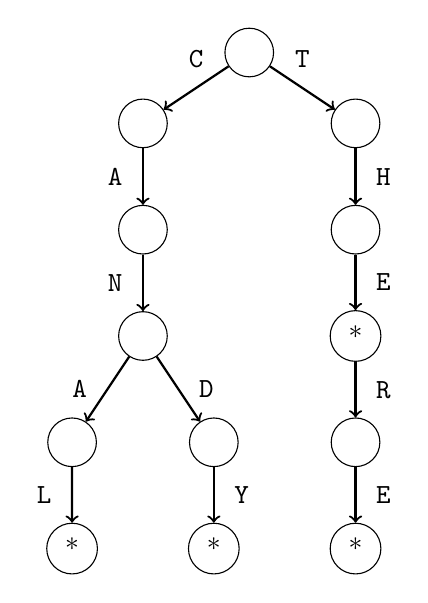
\begin{tikzpicture}[scale=0.9]
\node[draw, circle] (1) at (0,20) {$\phantom{1}$};
\node[draw, circle] (2) at (-1.5,19) {$\phantom{1}$};
\node[draw, circle] (3) at (1.5,19) {$\phantom{1}$};
\node[draw, circle] (4) at (-1.5,17.5) {$\phantom{1}$};
\node[draw, circle] (5) at (-1.5,16) {$\phantom{1}$};
\node[draw, circle] (6) at (-2.5,14.5) {$\phantom{1}$};
\node[draw, circle] (7) at (-0.5,14.5) {$\phantom{1}$};
\node[draw, circle] (8) at (-2.5,13) {*};
\node[draw, circle] (9) at (-0.5,13) {*};
\node[draw, circle] (10) at (1.5,17.5) {$\phantom{1}$};
\node[draw, circle] (11) at (1.5,16) {*};
\node[draw, circle] (12) at (1.5,14.5) {$\phantom{1}$};
\node[draw, circle] (13) at (1.5,13) {*};

\path[draw,thick,->] (1) -- node[font=\small,label=\texttt{C}] {} (2);
\path[draw,thick,->] (1) -- node[font=\small,label=\texttt{T}] {} (3);
\path[draw,thick,->] (2) -- node[font=\small,label=left:\texttt{A}] {} (4);
\path[draw,thick,->] (4) -- node[font=\small,label=left:\texttt{N}] {} (5);
\path[draw,thick,->] (5) -- node[font=\small,label=left:\texttt{A}] {} (6);
\path[draw,thick,->] (5) -- node[font=\small,label=right:\texttt{D}] {} (7);
\path[draw,thick,->] (6) -- node[font=\small,label=left:\texttt{L}] {}(8);
\path[draw,thick,->] (7) -- node[font=\small,label=right:\texttt{Y}] {} (9);
\path[draw,thick,->] (3) -- node[font=\small,label=right:\texttt{H}] {} (10);
\path[draw,thick,->] (10) -- node[font=\small,label=right:\texttt{E}] {} (11);
\path[draw,thick,->] (11) -- node[font=\small,label=right:\texttt{R}] {} (12);
\path[draw,thick,->] (12) -- node[font=\small,label=right:\texttt{E}] {} (13);
\end{tikzpicture}
\end{center}
The character * in a node means that
a string ends at the node.
This character is needed because a string
may be a prefix of another string.
For example, in this trie, \texttt{THE}
is a suffix of \texttt{THERE}.

Inserting and searching a string in a trie take $O(n)$ time
where $n$ is the length of the string.
Both operations can be implemented by
starting at the root node and following the
chain of characters that appear in the string.
If needed, new nodes will be added to the trie.

Trie can be used for searching both strings
and prefixes of strings.
In addition, we can keep track of the number
of strings that have each prefix,
that can be useful in some applications.

A trie can be stored as an array
\begin{lstlisting}
int t[N][A];
\end{lstlisting}
where $N$ is the maximum number of nodes
(the total length of the string to be stored)
and $A$ is the size of the alphabet.
The nodes of a trie are numbered
$1,2,3,\ldots$ so that the number of the root is 1,
and $\texttt{t}[s][c]$ is the next node in chain
from node $s$ using character $c$.

\section{Merkkijonohajautus}

\index{hajautus@hajautus}
\index{merkkijonohajautus@merkkijonohajautus}

\key{Merkkijonohajautus}
on tekniikka, jonka avulla voi esikäsittelyn
jälkeen tarkastaa tehokkaasti, ovatko
kaksi merkkijonon osajonoa samat.
Ideana on verrata toisiinsa
osajonojen hajautusarvoja,
mikä on tehokkaampaa kuin osajonojen
vertaaminen merkki kerrallaan.

\subsubsection*{Hajautusarvon laskeminen}

\index{hajautusarvo@hajautusarvo}
\index{polynominen hajautus@polynominen hajautus}

Merkkijonon \key{hajautusarvo}
on luku, joka lasketaan merkkijonon merkeistä
etukäteen valitulla tavalla.
Jos kaksi merkkijonoa ovat samat,
myös niiden hajautusarvot ovat samat,
minkä ansiosta merkkijonoja voi vertailla
niiden hajautusarvojen kautta.

Tavallinen tapa toteuttaa merkkijonohajautus
on käyttää polynomista hajautusta.
Siinä hajautusarvo lasketaan kaavalla
\[(c[1] A^{n-1} + c[2] A^{n-2} + \cdots + c[n] A^0) \bmod B  ,\]
missä merkkijonon merkkien koodit ovat
$c[1],c[2],\ldots,c[n]$ ja $A$ ja $B$ ovat etukäteen
valitut vakiot.

Esimerkiksi merkkijonon \texttt{KISSA} merkkien koodit ovat:
\begin{center}
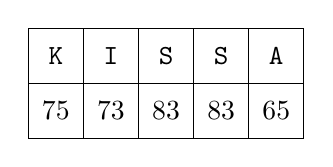
\begin{tikzpicture}[scale=0.7]
\draw (0,0) grid (5,2);

\node at (0.5, 1.5) {\texttt{K}};
\node at (1.5, 1.5) {\texttt{I}};
\node at (2.5, 1.5) {\texttt{S}};
\node at (3.5, 1.5) {\texttt{S}};
\node at (4.5, 1.5) {\texttt{A}};

\node at (0.5, 0.5) {75};
\node at (1.5, 0.5) {73};
\node at (2.5, 0.5) {83};
\node at (3.5, 0.5) {83};
\node at (4.5, 0.5) {65};

\end{tikzpicture}
\end{center}

Jos $A=3$ ja $B=97$, merkkijonon \texttt{KISSA} hajautusarvoksi tulee

\[(75 \cdot 3^4 + 73 \cdot 3^3 + 83 \cdot 3^2 + 83 \cdot 3^1 + 65 \cdot 3^0) \bmod 97 = 59.\]

\subsubsection*{Esikäsittely}

Merkkijonohajautuksen esikäsittely
muodostaa tietoa, jonka avulla 
voi laskea tehokkaasti merkkijonon
osajonojen hajautusarvoja.
Osoittautuu, että polynomisessa hajautuksessa
$O(n)$-aikaisen esikäsittelyn jälkeen voi laskea
minkä tahansa osajonon hajautusarvon
ajassa $O(1)$.

Ideana on muodostaa taulukko $h$,
jossa $h[k]$ on hajautusarvo merkkijonon
alkuosalle kohtaan $k$ asti.
Taulukon voi muodostaa rekursiolla seuraavasti:
\[
\begin{array}{lcl}
h[0] & = & 0 \\
h[k] & = & (h[k-1] A + c[k]) \bmod B \\
\end{array}
\]
Lisäksi muodostetaan taulukko $p$,
jossa $p[k]=A^k \bmod B$:
\[
\begin{array}{lcl}
p[0] & = & 1 \\
p[k] & = & (p[k-1] A) \bmod B. \\
\end{array}
\]
Näiden taulukoiden muodostaminen vie aikaa $O(n)$.
Tämän jälkeen hajautusarvo merkkijonon osajonolle,
joka alkaa kohdasta $a$ ja päättyy kohtaan $b$,
voidaan laskea $O(1)$-ajassa kaavalla
\[(h[b]-h[a-1] p[b-a+1]) \bmod B.\]

\subsubsection*{Hajautuksen käyttö}

Hajautusarvot tarjoavat nopean tavan merkkijonojen
vertailemiseen.
Ideana on vertailla merkkijonojen koko sisällön
sijasta niiden hajautusarvoja.
Jos hajautusarvot ovat samat,
myös merkkijonot ovat \textit{todennäköisesti} samat,
ja jos taas hajautusarvot eivät ole samat,
merkkijonot eivät \textit{varmasti} ole samat.

Hajautuksen avulla voi usein tehostaa
raa'an voiman algoritmia niin, että siitä tulee tehokas.
Tarkastellaan esimerkkinä
raa'an voiman algoritmia, joka laskee,
montako kertaa merkkijono $p$
esiintyy osajonona merkkijonossa $s$.
Algoritmi käy läpi kaikki kohdat,
joissa $p$ voi esiintyä,
ja vertailee merkkijonoja merkki merkiltä.
Tällaisen algoritmin aikavaativuus on $O(n^2)$.

Voimme kuitenkin tehostaa algoritmia hajautuksen avulla,
koska algoritmissa vertaillaan merkkijonojen osajonoja.
Hajautusta käyttäen kukin vertailu vie aikaa vain $O(1)$,
koska vertailua ei tehdä merkki merkiltä
vaan suoraan hajautusarvon perusteella.
Tuloksena on algoritmi, jonka aikavaativuus on $O(n)$,
joka on paras mahdollinen aikavaativuus tehtävään.

Yhdistämällä hajautus ja \emph{binäärihaku} on mahdollista
myös selvittää logaritmisessa ajassa,
kumpi kahdesta osajonosta on suurempi
aakkosjärjestyksessä.
Tämä onnistuu tutkimalla ensin binäärihaulla,
kuinka pitkä on merkkijonojen yhteinen alkuosa,
minkä jälkeen yhteisen alkuosan jälkeinen merkki
kertoo, kumpi merkkijono on suurempi.

\subsubsection*{Törmäykset ja parametrit}

\index{tzzmxys@törmäys}

Ilmeinen riski hajautusarvojen vertailussa
on \key{törmäys}, joka tarkoittaa, että kahdessa merkkijonossa on
eri sisältö mutta niiden hajautusarvot ovat samat.
Tällöin hajautusarvojen perusteella merkkijonot
näyttävät samalta, vaikka todellisuudessa ne eivät ole samat,
ja algoritmi voi toimia väärin.

Törmäyksen riski on aina olemassa,
koska erilaisia merkkijonoja on enemmän kuin
erilaisia hajautusarvoja.
Riskin saa kuitenkin pieneksi valitsemalla
hajautuksen vakiot $A$ ja $B$ huolellisesti.
Vakioiden valinnassa on kaksi tavoitetta:
hajautusarvojen tulisi
jakautua tasaisesti merkkijonoille
ja
erilaisten hajautusarvojen määrän tulisi
olla riittävän suuri.

Hyvä ratkaisu on valita vakioiksi suuria
satunnaislukuja. Tavallinen tapa on valita vakiot
läheltä lukua $10^9$, esimerkiksi
\[
\begin{array}{lcl}
A & = & 911382323 \\
B & = & 972663749 \\
\end{array}
\]
Tällainen valinta takaa sen,
että hajautusarvot jakautuvat
riittävän tasaisesti välille $0 \ldots B-1$.
Suuruusluokan $10^9$ etuna on,
että \texttt{long long} -tyyppi riittää
hajautusarvojen käsittelyyn koodissa,
koska tulot $AB$ ja $BB$ mahtuvat \texttt{long long} -tyyppiin.
Mutta onko $10^9$ riittävä määrä hajautusarvoja?

Tarkastellaan nyt kolmea hajautuksen käyttötapaa:

\textit{Tapaus 1:} Merkkijonoja $x$ ja $y$ verrataan toisiinsa.
Törmäyksen todennäköisyys on $1/B$ olettaen,
että kaikki hajautusarvot esiintyvät yhtä usein.

\textit{Tapaus 2:} Merkkijonoa $x$ verrataan merkkijonoihin
$y_1,y_2,\ldots,y_n$.
Yhden tai useamman törmäyksen todennäköisyys on

\[1-(1-1/B)^n.\]

\textit{Tapaus 3:} Merkkijonoja $x_1,x_2,\ldots,x_n$
verrataan kaikkia keskenään.
Yhden tai useamman törmäyksen todennäköisyys on
\[ 1 - \frac{B \cdot (B-1) \cdot (B-2) \cdots (B-n+1)}{B^n}.\]

Seuraava taulukko sisältää törmäyksen todennäköisyydet,
kun vakion $B$ arvo vaihtelee ja $n=10^6$:

\begin{center}
\begin{tabular}{rrrr}
vakio $B$ & tapaus 1 & tapaus 2 & tapaus 3 \\
\hline
$10^3$ & $0.001000$ & $1.000000$ & $1.000000$ \\
$10^6$ & $0.000001$ & $0.632121$ & $1.000000$ \\
$10^9$ & $0.000000$ & $0.001000$ & $1.000000$ \\
$10^{12}$ & $0.000000$ & $0.000000$ & $0.393469$ \\
$10^{15}$ & $0.000000$ & $0.000000$ & $0.000500$ \\
$10^{18}$ & $0.000000$ & $0.000000$ & $0.000001$ \\
\end{tabular}
\end{center}

Taulukosta näkee, että tapauksessa 1
törmäyksen riski on olematon
valinnalla $B \approx 10^9$.
Tapauksessa 2 riski on olemassa, mutta se on silti edelleen vähäinen.
Tapauksessa 3 tilanne on kuitenkin täysin toinen:
törmäys tapahtuu käytännössä varmasti
vielä valinnalla $B \approx 10^9$.

\index{syntymxpxivxparadoksi@syntymäpäiväparadoksi}

Tapauksen 3 ilmiö tunnetaan nimellä
\key{syntymäpäiväparadoksi}:
jos huoneessa on $n$ henkilöä, on suuri
todennäköisyys, että jollain kahdella
henkilöllä on sama syntymäpäivä, vaikka
$n$ olisi melko pieni.
Vastaavasti hajautuksessa kun kaikkia
hajautusarvoja verrataan keskenään,
käy helposti niin, että jotkin
kaksi ovat sattumalta samoja.

Hyvä tapa pienentää törmäyksen riskiä on laskea
\emph{useita} hajautusarvoja eri parametreilla
ja verrata niitä kaikkia.
On hyvin pieni todennäköisyys,
että törmäys tapahtuisi samaan aikaan
kaikissa hajautusarvoissa.
Esimerkiksi kaksi hajautusarvoa parametrilla
$B \approx 10^9$ vastaa yhtä hajautusarvoa
parametrilla $B \approx 10^{18}$,
mikä takaa hyvän suojan törmäyksiltä.

Jotkut käyttävät hajautuksessa vakioita $B=2^{32}$ tai $B=2^{64}$,
jolloin modulo $B$ tulee laskettua
automaattisesti, kun muuttujan arvo pyörähtää ympäri.
Tämä ei ole kuitenkaan hyvä valinta,
koska muotoa $2^x$ olevaa moduloa vastaan
pystyy tekemään testisyötteen, joka aiheuttaa varmasti törmäyksen\footnote{
J. Pachocki ja Jakub Radoszweski:
''Where to use and how not to use polynomial string hashing''.
\textit{Olympiads in Informatics}, 2013.
}.

\section{Z-algoritmi}

\index{Z-algoritmi}
\index{Z-taulukko}

\key{Z-algoritmi} muodostaa merkkijonosta \key{Z-taulukon},
joka kertoo kullekin merkkijonon kohdalle,
mikä on pisin kyseisestä kohdasta alkava osajono,
joka on myös merkkijonon alkuosa.
Z-algoritmin avulla voi ratkaista tehokkaasti
monia merkkijonotehtäviä.

Z-algoritmi ja merkkijonohajautus ovat usein
vaihtoehtoisia tekniikoita, ja on makuasia,
kumpaa algoritmia käyttää.
Toisin kuin hajautus, Z-algoritmi toimii
varmasti oikein eikä siinä ole törmäysten riskiä.
Toisaalta Z-algoritmi on vaikeampi toteuttaa eikä
se sovellu kaikkeen samaan kuin hajautus.

\subsubsection*{Algoritmin toiminta}

Z-algoritmi muodostaa merkkijonolle Z-taulukon,
jonka jokaisessa kohdassa lukee,
kuinka pitkälle kohdasta
alkava osajono vastaa merkkijonon alkuosaa.
Esimerkiksi Z-taulukko
merkkijonolle \texttt{ACBACDACBACBACDA} on seuraava:

\begin{center}
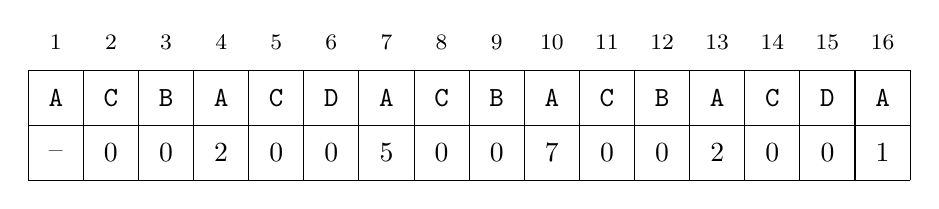
\begin{tikzpicture}[scale=0.7]
\draw (0,0) grid (16,2);

\node at (0.5, 1.5) {\texttt{A}};
\node at (1.5, 1.5) {\texttt{C}};
\node at (2.5, 1.5) {\texttt{B}};
\node at (3.5, 1.5) {\texttt{A}};
\node at (4.5, 1.5) {\texttt{C}};
\node at (5.5, 1.5) {\texttt{D}};
\node at (6.5, 1.5) {\texttt{A}};
\node at (7.5, 1.5) {\texttt{C}};
\node at (8.5, 1.5) {\texttt{B}};
\node at (9.5, 1.5) {\texttt{A}};
\node at (10.5, 1.5) {\texttt{C}};
\node at (11.5, 1.5) {\texttt{B}};
\node at (12.5, 1.5) {\texttt{A}};
\node at (13.5, 1.5) {\texttt{C}};
\node at (14.5, 1.5) {\texttt{D}};
\node at (15.5, 1.5) {\texttt{A}};

\node at (0.5, 0.5) {--};
\node at (1.5, 0.5) {0};
\node at (2.5, 0.5) {0};
\node at (3.5, 0.5) {2};
\node at (4.5, 0.5) {0};
\node at (5.5, 0.5) {0};
\node at (6.5, 0.5) {5};
\node at (7.5, 0.5) {0};
\node at (8.5, 0.5) {0};
\node at (9.5, 0.5) {7};
\node at (10.5, 0.5) {0};
\node at (11.5, 0.5) {0};
\node at (12.5, 0.5) {2};
\node at (13.5, 0.5) {0};
\node at (14.5, 0.5) {0};
\node at (15.5, 0.5) {1};

\footnotesize
\node at (0.5, 2.5) {1};
\node at (1.5, 2.5) {2};
\node at (2.5, 2.5) {3};
\node at (3.5, 2.5) {4};
\node at (4.5, 2.5) {5};
\node at (5.5, 2.5) {6};
\node at (6.5, 2.5) {7};
\node at (7.5, 2.5) {8};
\node at (8.5, 2.5) {9};
\node at (9.5, 2.5) {10};
\node at (10.5, 2.5) {11};
\node at (11.5, 2.5) {12};
\node at (12.5, 2.5) {13};
\node at (13.5, 2.5) {14};
\node at (14.5, 2.5) {15};
\node at (15.5, 2.5) {16};

\end{tikzpicture}
\end{center}

Esimerkiksi kohdassa 7 on arvo 5,
koska siitä alkava 5-merkkinen osajono
\texttt{ACBAC} on merkkijonon alkuosa,
mutta 6-merkkinen osajono \texttt{ACBACB}
ei ole enää merkkijonon alkuosa.

Z-algoritmi käy läpi merkkijonon
vasemmalta oikealle ja laskee
jokaisessa kohdassa,
kuinka pitkälle kyseisestä kohdasta alkava
osajono täsmää merkkijonon alkuun.
Algoritmi laskee yhteisen
alkuosan pituuden vertaamalla
merkkijonon alkua ja osajonon alkua toisiinsa.

Suoraviivaisesti toteutettuna
tällaisen algoritmin aikavaativuus olisi $O(n^2)$,
koska yhteiset alkuosat voivat olla pitkiä.
Z-algoritmissa on kuitenkin yksi tärkeä
optimointi, jonka ansiosta algoritmin
aikavaativuus on vain $O(n)$.

Ideana on pitää muistissa väliä $[x,y]$,
joka on aiemmin laskettu merkkijonon
alkuun täsmäävä väli, jossa $y$ on 
mahdollisimman suuri.
Tällä välillä olevia
merkkejä ei tarvitse koskaan
verrata uudestaan
merkkijonon alkuun, vaan niitä koskevan
tiedon saa suoraan Z-taulukon lasketusta osasta.

Z-algoritmin aikavaativuus on $O(n)$,
koska algoritmi aloittaa merkki kerrallaan
vertailemisen vasta kohdasta $y+1$.
Jos merkit täsmäävät, kohta $y$
siirtyy eteenpäin
eikä algoritmin tarvitse enää
koskaan vertailla tätä kohtaa,
vaan algoritmi pystyy hyödyntämään
Z-taulukon alussa olevaa tietoa.

\subsubsection*{Esimerkki}

Katsotaan nyt, miten Z-algoritmi muodostaa
seuraavan Z-taulukon:

\begin{center}
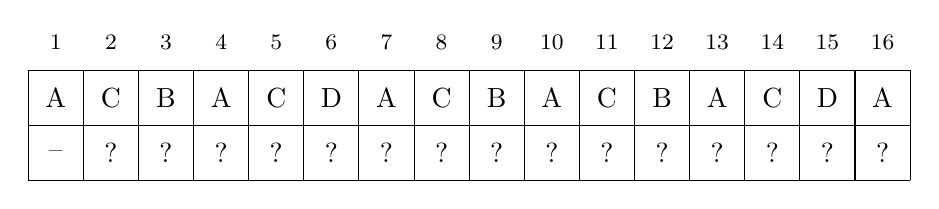
\begin{tikzpicture}[scale=0.7]
\draw (0,0) grid (16,2);

\node at (0.5, 1.5) {A};
\node at (1.5, 1.5) {C};
\node at (2.5, 1.5) {B};
\node at (3.5, 1.5) {A};
\node at (4.5, 1.5) {C};
\node at (5.5, 1.5) {D};
\node at (6.5, 1.5) {A};
\node at (7.5, 1.5) {C};
\node at (8.5, 1.5) {B};
\node at (9.5, 1.5) {A};
\node at (10.5, 1.5) {C};
\node at (11.5, 1.5) {B};
\node at (12.5, 1.5) {A};
\node at (13.5, 1.5) {C};
\node at (14.5, 1.5) {D};
\node at (15.5, 1.5) {A};

\node at (0.5, 0.5) {--};
\node at (1.5, 0.5) {?};
\node at (2.5, 0.5) {?};
\node at (3.5, 0.5) {?};
\node at (4.5, 0.5) {?};
\node at (5.5, 0.5) {?};
\node at (6.5, 0.5) {?};
\node at (7.5, 0.5) {?};
\node at (8.5, 0.5) {?};
\node at (9.5, 0.5) {?};
\node at (10.5, 0.5) {?};
\node at (11.5, 0.5) {?};
\node at (12.5, 0.5) {?};
\node at (13.5, 0.5) {?};
\node at (14.5, 0.5) {?};
\node at (15.5, 0.5) {?};

\footnotesize
\node at (0.5, 2.5) {1};
\node at (1.5, 2.5) {2};
\node at (2.5, 2.5) {3};
\node at (3.5, 2.5) {4};
\node at (4.5, 2.5) {5};
\node at (5.5, 2.5) {6};
\node at (6.5, 2.5) {7};
\node at (7.5, 2.5) {8};
\node at (8.5, 2.5) {9};
\node at (9.5, 2.5) {10};
\node at (10.5, 2.5) {11};
\node at (11.5, 2.5) {12};
\node at (12.5, 2.5) {13};
\node at (13.5, 2.5) {14};
\node at (14.5, 2.5) {15};
\node at (15.5, 2.5) {16};

\end{tikzpicture}
\end{center}

Ensimmäinen mielenkiintoinen kohta tulee,
kun yhteisen alkuosan pituus on 5.
Silloin algoritmi laittaa muistiin
välin $[7,11]$ seuraavasti:

\begin{center}
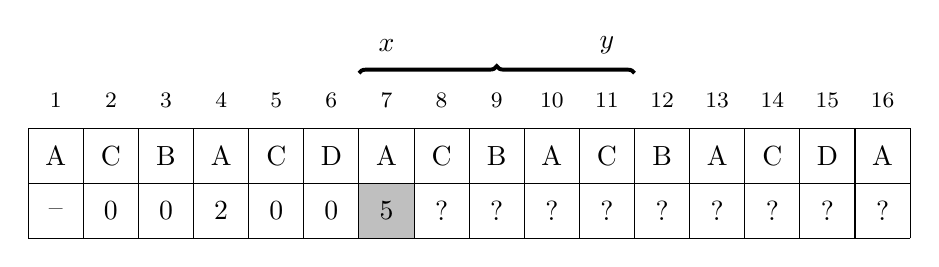
\begin{tikzpicture}[scale=0.7]
\fill[color=lightgray] (6,0) rectangle (7,1);
\draw (0,0) grid (16,2);

\node at (0.5, 1.5) {A};
\node at (1.5, 1.5) {C};
\node at (2.5, 1.5) {B};
\node at (3.5, 1.5) {A};
\node at (4.5, 1.5) {C};
\node at (5.5, 1.5) {D};
\node at (6.5, 1.5) {A};
\node at (7.5, 1.5) {C};
\node at (8.5, 1.5) {B};
\node at (9.5, 1.5) {A};
\node at (10.5, 1.5) {C};
\node at (11.5, 1.5) {B};
\node at (12.5, 1.5) {A};
\node at (13.5, 1.5) {C};
\node at (14.5, 1.5) {D};
\node at (15.5, 1.5) {A};

\node at (0.5, 0.5) {--};
\node at (1.5, 0.5) {0};
\node at (2.5, 0.5) {0};
\node at (3.5, 0.5) {2};
\node at (4.5, 0.5) {0};
\node at (5.5, 0.5) {0};
\node at (6.5, 0.5) {5};
\node at (7.5, 0.5) {?};
\node at (8.5, 0.5) {?};
\node at (9.5, 0.5) {?};
\node at (10.5, 0.5) {?};
\node at (11.5, 0.5) {?};
\node at (12.5, 0.5) {?};
\node at (13.5, 0.5) {?};
\node at (14.5, 0.5) {?};
\node at (15.5, 0.5) {?};

\draw [decoration={brace}, decorate, line width=0.5mm] (6,3.00) -- (11,3.00);

\node at (6.5,3.50) {$x$};
\node at (10.5,3.50) {$y$};


\footnotesize
\node at (0.5, 2.5) {1};
\node at (1.5, 2.5) {2};
\node at (2.5, 2.5) {3};
\node at (3.5, 2.5) {4};
\node at (4.5, 2.5) {5};
\node at (5.5, 2.5) {6};
\node at (6.5, 2.5) {7};
\node at (7.5, 2.5) {8};
\node at (8.5, 2.5) {9};
\node at (9.5, 2.5) {10};
\node at (10.5, 2.5) {11};
\node at (11.5, 2.5) {12};
\node at (12.5, 2.5) {13};
\node at (13.5, 2.5) {14};
\node at (14.5, 2.5) {15};
\node at (15.5, 2.5) {16};

\end{tikzpicture}
\end{center}

Välin $[7,11]$ hyötynä on, että algoritmi
voi sen avulla laskea seuraavat
Z-taulukon arvot nopeammin.
Koska välin $[7,11]$ merkit ovat samat
kuin merkkijonon alussa,
myös Z-taulukon arvoissa on vastaavuutta.

Ensinnäkin kohdissa 8 ja 9
tulee olla samat arvot kuin
kohdissa 2 ja 3,
koska väli $[7,11]$
vastaa väliä $[1,5]$:

\begin{center}
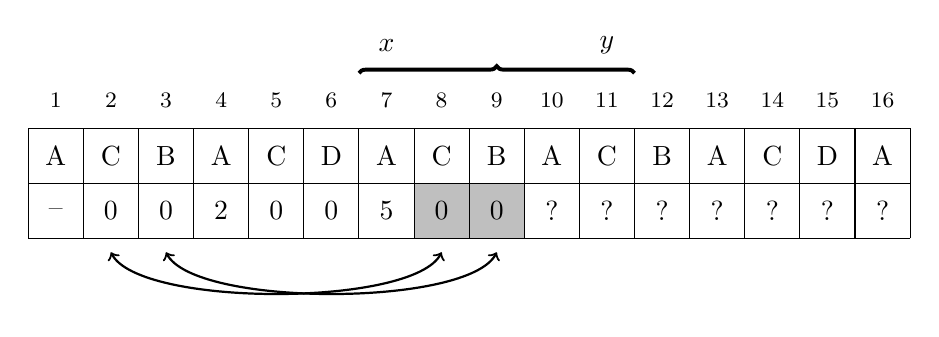
\begin{tikzpicture}[scale=0.7]
\fill[color=lightgray] (7,0) rectangle (9,1);
\draw (0,0) grid (16,2);

\node at (0.5, 1.5) {A};
\node at (1.5, 1.5) {C};
\node at (2.5, 1.5) {B};
\node at (3.5, 1.5) {A};
\node at (4.5, 1.5) {C};
\node at (5.5, 1.5) {D};
\node at (6.5, 1.5) {A};
\node at (7.5, 1.5) {C};
\node at (8.5, 1.5) {B};
\node at (9.5, 1.5) {A};
\node at (10.5, 1.5) {C};
\node at (11.5, 1.5) {B};
\node at (12.5, 1.5) {A};
\node at (13.5, 1.5) {C};
\node at (14.5, 1.5) {D};
\node at (15.5, 1.5) {A};

\node at (0.5, 0.5) {--};
\node at (1.5, 0.5) {0};
\node at (2.5, 0.5) {0};
\node at (3.5, 0.5) {2};
\node at (4.5, 0.5) {0};
\node at (5.5, 0.5) {0};
\node at (6.5, 0.5) {5};
\node at (7.5, 0.5) {0};
\node at (8.5, 0.5) {0};
\node at (9.5, 0.5) {?};
\node at (10.5, 0.5) {?};
\node at (11.5, 0.5) {?};
\node at (12.5, 0.5) {?};
\node at (13.5, 0.5) {?};
\node at (14.5, 0.5) {?};
\node at (15.5, 0.5) {?};


\draw [decoration={brace}, decorate, line width=0.5mm] (6,3.00) -- (11,3.00);

\node at (6.5,3.50) {$x$};
\node at (10.5,3.50) {$y$};


\footnotesize
\node at (0.5, 2.5) {1};
\node at (1.5, 2.5) {2};
\node at (2.5, 2.5) {3};
\node at (3.5, 2.5) {4};
\node at (4.5, 2.5) {5};
\node at (5.5, 2.5) {6};
\node at (6.5, 2.5) {7};
\node at (7.5, 2.5) {8};
\node at (8.5, 2.5) {9};
\node at (9.5, 2.5) {10};
\node at (10.5, 2.5) {11};
\node at (11.5, 2.5) {12};
\node at (12.5, 2.5) {13};
\node at (13.5, 2.5) {14};
\node at (14.5, 2.5) {15};
\node at (15.5, 2.5) {16};


\draw[thick,<->] (7.5,-0.25) .. controls (7,-1.25) and (2,-1.25) .. (1.5,-0.25);
\draw[thick,<->] (8.5,-0.25) .. controls (8,-1.25) and (3,-1.25) .. (2.5,-0.25);
\end{tikzpicture}
\end{center}

Seuraavaksi kohdasta 4 saa tietoa kohdan
10 arvon laskemiseksi.
Koska kohdassa 4 on arvo 2,
tämä tarkoittaa, että osajono
täsmää kohtaan $y=11$ asti,
mutta sen jälkeen on tutkimatonta
aluetta merkkijonossa.

\begin{center}
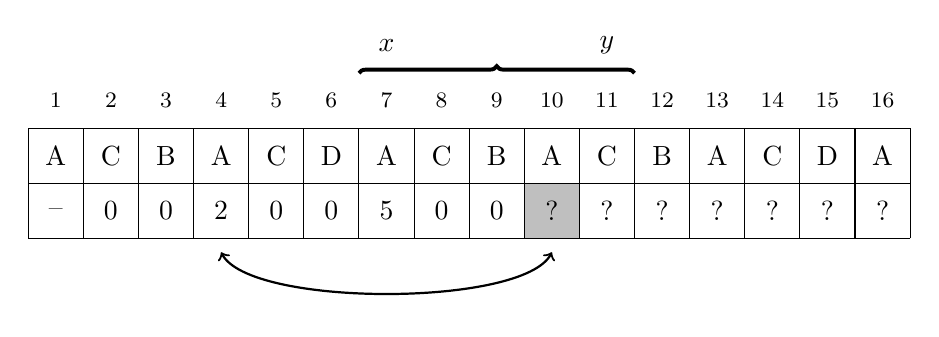
\begin{tikzpicture}[scale=0.7]
\fill[color=lightgray] (9,0) rectangle (10,1);
\draw (0,0) grid (16,2);

\node at (0.5, 1.5) {A};
\node at (1.5, 1.5) {C};
\node at (2.5, 1.5) {B};
\node at (3.5, 1.5) {A};
\node at (4.5, 1.5) {C};
\node at (5.5, 1.5) {D};
\node at (6.5, 1.5) {A};
\node at (7.5, 1.5) {C};
\node at (8.5, 1.5) {B};
\node at (9.5, 1.5) {A};
\node at (10.5, 1.5) {C};
\node at (11.5, 1.5) {B};
\node at (12.5, 1.5) {A};
\node at (13.5, 1.5) {C};
\node at (14.5, 1.5) {D};
\node at (15.5, 1.5) {A};

\node at (0.5, 0.5) {--};
\node at (1.5, 0.5) {0};
\node at (2.5, 0.5) {0};
\node at (3.5, 0.5) {2};
\node at (4.5, 0.5) {0};
\node at (5.5, 0.5) {0};
\node at (6.5, 0.5) {5};
\node at (7.5, 0.5) {0};
\node at (8.5, 0.5) {0};
\node at (9.5, 0.5) {?};
\node at (10.5, 0.5) {?};
\node at (11.5, 0.5) {?};
\node at (12.5, 0.5) {?};
\node at (13.5, 0.5) {?};
\node at (14.5, 0.5) {?};
\node at (15.5, 0.5) {?};

\draw [decoration={brace}, decorate, line width=0.5mm] (6,3.00) -- (11,3.00);

\node at (6.5,3.50) {$x$};
\node at (10.5,3.50) {$y$};


\footnotesize
\node at (0.5, 2.5) {1};
\node at (1.5, 2.5) {2};
\node at (2.5, 2.5) {3};
\node at (3.5, 2.5) {4};
\node at (4.5, 2.5) {5};
\node at (5.5, 2.5) {6};
\node at (6.5, 2.5) {7};
\node at (7.5, 2.5) {8};
\node at (8.5, 2.5) {9};
\node at (9.5, 2.5) {10};
\node at (10.5, 2.5) {11};
\node at (11.5, 2.5) {12};
\node at (12.5, 2.5) {13};
\node at (13.5, 2.5) {14};
\node at (14.5, 2.5) {15};
\node at (15.5, 2.5) {16};

\draw[thick,<->] (9.5,-0.25) .. controls (9,-1.25) and (4,-1.25) .. (3.5,-0.25);
\end{tikzpicture}
\end{center}

Nyt algoritmi alkaa vertailla merkkejä
kohdasta $y+1=12$ alkaen merkki kerrallaan.
Algoritmi ei voi hyödyntää valmiina
Z-taulukossa olevaa tietoa, koska se ei ole vielä aiemmin
tutkinut merkkijonoa näin pitkälle.
Tuloksena osajonon pituudeksi tulee 7
ja väli $[x,y]$ päivittyy vastaavasti:

\begin{center}
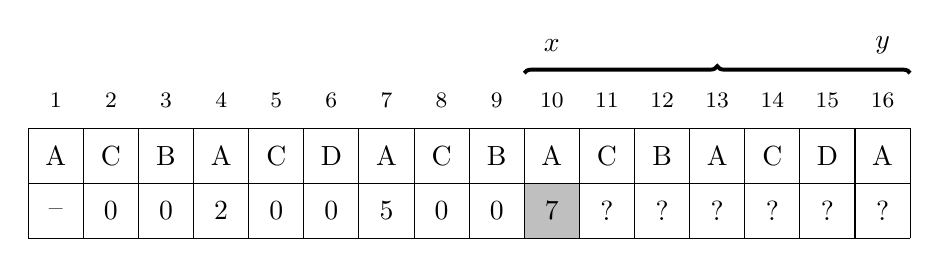
\begin{tikzpicture}[scale=0.7]
\fill[color=lightgray] (9,0) rectangle (10,1);
\draw (0,0) grid (16,2);

\node at (0.5, 1.5) {A};
\node at (1.5, 1.5) {C};
\node at (2.5, 1.5) {B};
\node at (3.5, 1.5) {A};
\node at (4.5, 1.5) {C};
\node at (5.5, 1.5) {D};
\node at (6.5, 1.5) {A};
\node at (7.5, 1.5) {C};
\node at (8.5, 1.5) {B};
\node at (9.5, 1.5) {A};
\node at (10.5, 1.5) {C};
\node at (11.5, 1.5) {B};
\node at (12.5, 1.5) {A};
\node at (13.5, 1.5) {C};
\node at (14.5, 1.5) {D};
\node at (15.5, 1.5) {A};

\node at (0.5, 0.5) {--};
\node at (1.5, 0.5) {0};
\node at (2.5, 0.5) {0};
\node at (3.5, 0.5) {2};
\node at (4.5, 0.5) {0};
\node at (5.5, 0.5) {0};
\node at (6.5, 0.5) {5};
\node at (7.5, 0.5) {0};
\node at (8.5, 0.5) {0};
\node at (9.5, 0.5) {7};
\node at (10.5, 0.5) {?};
\node at (11.5, 0.5) {?};
\node at (12.5, 0.5) {?};
\node at (13.5, 0.5) {?};
\node at (14.5, 0.5) {?};
\node at (15.5, 0.5) {?};

\draw [decoration={brace}, decorate, line width=0.5mm] (9,3.00) -- (16,3.00);

\node at (9.5,3.50) {$x$};
\node at (15.5,3.50) {$y$};


\footnotesize
\node at (0.5, 2.5) {1};
\node at (1.5, 2.5) {2};
\node at (2.5, 2.5) {3};
\node at (3.5, 2.5) {4};
\node at (4.5, 2.5) {5};
\node at (5.5, 2.5) {6};
\node at (6.5, 2.5) {7};
\node at (7.5, 2.5) {8};
\node at (8.5, 2.5) {9};
\node at (9.5, 2.5) {10};
\node at (10.5, 2.5) {11};
\node at (11.5, 2.5) {12};
\node at (12.5, 2.5) {13};
\node at (13.5, 2.5) {14};
\node at (14.5, 2.5) {15};
\node at (15.5, 2.5) {16};

% \draw[thick,<->] (9.5,-0.25) .. controls (9,-1.25) and (4,-1.25) .. (3.5,-0.25);
\end{tikzpicture}
\end{center}

Tämän jälkeen kaikkien seuraavien Z-taulukon
arvojen laskemisessa pystyy hyödyntämään
jälleen välin $[x,y]$ antamaa tietoa
ja algoritmi saa Z-taulukon loppuun tulevat
arvot suoraan Z-taulukon alusta:

\begin{center}
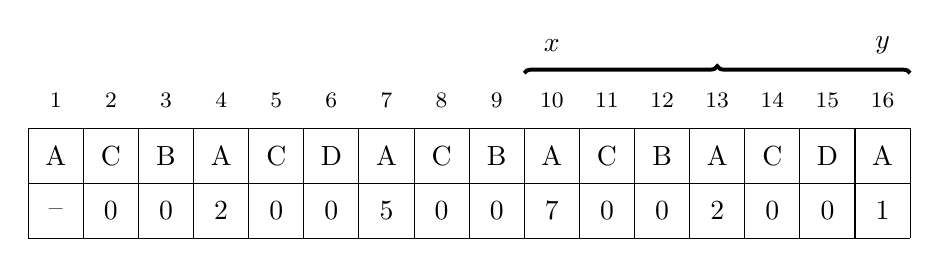
\begin{tikzpicture}[scale=0.7]
\draw (0,0) grid (16,2);

\node at (0.5, 1.5) {A};
\node at (1.5, 1.5) {C};
\node at (2.5, 1.5) {B};
\node at (3.5, 1.5) {A};
\node at (4.5, 1.5) {C};
\node at (5.5, 1.5) {D};
\node at (6.5, 1.5) {A};
\node at (7.5, 1.5) {C};
\node at (8.5, 1.5) {B};
\node at (9.5, 1.5) {A};
\node at (10.5, 1.5) {C};
\node at (11.5, 1.5) {B};
\node at (12.5, 1.5) {A};
\node at (13.5, 1.5) {C};
\node at (14.5, 1.5) {D};
\node at (15.5, 1.5) {A};

\node at (0.5, 0.5) {--};
\node at (1.5, 0.5) {0};
\node at (2.5, 0.5) {0};
\node at (3.5, 0.5) {2};
\node at (4.5, 0.5) {0};
\node at (5.5, 0.5) {0};
\node at (6.5, 0.5) {5};
\node at (7.5, 0.5) {0};
\node at (8.5, 0.5) {0};
\node at (9.5, 0.5) {7};
\node at (10.5, 0.5) {0};
\node at (11.5, 0.5) {0};
\node at (12.5, 0.5) {2};
\node at (13.5, 0.5) {0};
\node at (14.5, 0.5) {0};
\node at (15.5, 0.5) {1};

\draw [decoration={brace}, decorate, line width=0.5mm] (9,3.00) -- (16,3.00);

\node at (9.5,3.50) {$x$};
\node at (15.5,3.50) {$y$};


\footnotesize
\node at (0.5, 2.5) {1};
\node at (1.5, 2.5) {2};
\node at (2.5, 2.5) {3};
\node at (3.5, 2.5) {4};
\node at (4.5, 2.5) {5};
\node at (5.5, 2.5) {6};
\node at (6.5, 2.5) {7};
\node at (7.5, 2.5) {8};
\node at (8.5, 2.5) {9};
\node at (9.5, 2.5) {10};
\node at (10.5, 2.5) {11};
\node at (11.5, 2.5) {12};
\node at (12.5, 2.5) {13};
\node at (13.5, 2.5) {14};
\node at (14.5, 2.5) {15};
\node at (15.5, 2.5) {16};

\end{tikzpicture}
\end{center}

\subsubsection{Z-taulukon käyttäminen}

Ratkaistaan esimerkkinä tehtävä,
jossa laskettavana on,
montako kertaa merkkijono $p$
esiintyy osajonona merkkijonossa $s$.
Ratkaisimme tehtävän aiemmin tehokkaasti
merkkijonohajautuksen avulla,
ja nyt Z-algoritmi tarjoaa siihen
vaihtoehtoisen lähestymistavan.

Usein esiintyvä idea Z-algoritmin yhteydessä
on muodostaa merkkijono,
jonka osana on useita välimerkeillä
erotettuja merkkijonoja.
Tässä tehtävässä sopiva merkkijono on
$p$\texttt{\#}$s$,
jossa merkkijonojen $p$ ja $s$ välissä on
erikoismerkki \texttt{\#},
jota ei esiinny merkkijonoissa.
Nyt merkkijonoa $p$\texttt{\#}$s$
vastaava Z-taulukko kertoo,
missä kohdissa merkkijonoa $p$
esiintyy merkkijono $s$.
Tällaiset kohdat ovat tarkalleen ne
Z-taulukon kohdat, joissa on
merkkijonon $p$ pituus.

\begin{samepage}
Esimerkiksi jos $s=$\texttt{HATTIVATTI} ja $p=$\texttt{ATT},
niin Z-taulukosta tulee:

\begin{center}
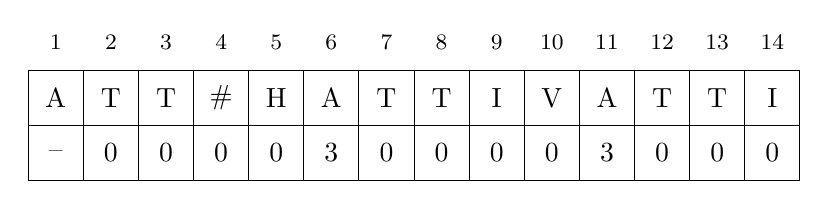
\begin{tikzpicture}[scale=0.7]
\draw (0,0) grid (14,2);

\node at (0.5, 1.5) {A};
\node at (1.5, 1.5) {T};
\node at (2.5, 1.5) {T};
\node at (3.5, 1.5) {\#};
\node at (4.5, 1.5) {H};
\node at (5.5, 1.5) {A};
\node at (6.5, 1.5) {T};
\node at (7.5, 1.5) {T};
\node at (8.5, 1.5) {I};
\node at (9.5, 1.5) {V};
\node at (10.5, 1.5) {A};
\node at (11.5, 1.5) {T};
\node at (12.5, 1.5) {T};
\node at (13.5, 1.5) {I};

\node at (0.5, 0.5) {--};
\node at (1.5, 0.5) {0};
\node at (2.5, 0.5) {0};
\node at (3.5, 0.5) {0};
\node at (4.5, 0.5) {0};
\node at (5.5, 0.5) {3};
\node at (6.5, 0.5) {0};
\node at (7.5, 0.5) {0};
\node at (8.5, 0.5) {0};
\node at (9.5, 0.5) {0};
\node at (10.5, 0.5) {3};
\node at (11.5, 0.5) {0};
\node at (12.5, 0.5) {0};
\node at (13.5, 0.5) {0};

\footnotesize
\node at (0.5, 2.5) {1};
\node at (1.5, 2.5) {2};
\node at (2.5, 2.5) {3};
\node at (3.5, 2.5) {4};
\node at (4.5, 2.5) {5};
\node at (5.5, 2.5) {6};
\node at (6.5, 2.5) {7};
\node at (7.5, 2.5) {8};
\node at (8.5, 2.5) {9};
\node at (9.5, 2.5) {10};
\node at (10.5, 2.5) {11};
\node at (11.5, 2.5) {12};
\node at (12.5, 2.5) {13};
\node at (13.5, 2.5) {14};
\end{tikzpicture}
\end{center}
\end{samepage}
Taulukon kohdissa 6 ja 11 on luku 3,
mikä tarkoittaa, että \texttt{ATT}
esiintyy vastaavissa kohdissa merkkijonossa
\texttt{HATTIVATTI}.

Tuloksena olevan algoritmin aikavaativuus on
$O(n)$, koska riittää muodostaa Z-taulukko
ja käydä se läpi.